% Editable reconstruction; interpretation recorded in root.json.
% Shared standalone design for the editable figure reconstructions.
\documentclass[tikz,border=5pt,10pt]{standalone}
\usepackage[T1]{fontenc}
\usepackage[utf8]{inputenc}
\usepackage{newpxtext,newpxmath}
\usepackage[scaled=.94]{sourcesanspro}
\usepackage{pgfplots}
\pgfplotsset{compat=1.18}
\usetikzlibrary{arrows.meta,calc,positioning,decorations.pathreplacing,
  decorations.markings,patterns,matrix,shapes.geometric,fit,backgrounds,
  intersections,angles,quotes}
\definecolor{ink}{HTML}{203746}
\definecolor{accent}{HTML}{146C78}
\definecolor{muted}{HTML}{667780}
\definecolor{signalred}{HTML}{B94B44}
\color{ink}
\tikzset{>=Latex,line width=.8pt,
  every node/.style={font=\small},
  axis/.style={->,draw=muted,line width=.5pt},
  guide/.style={draw=muted,dashed,line width=.45pt},
  curve/.style={draw=accent,line width=1pt},
  marker/.style={circle,fill=accent,inner sep=1.5pt},
  labelbox/.style={fill=white,inner sep=2pt}}

\begin{document}

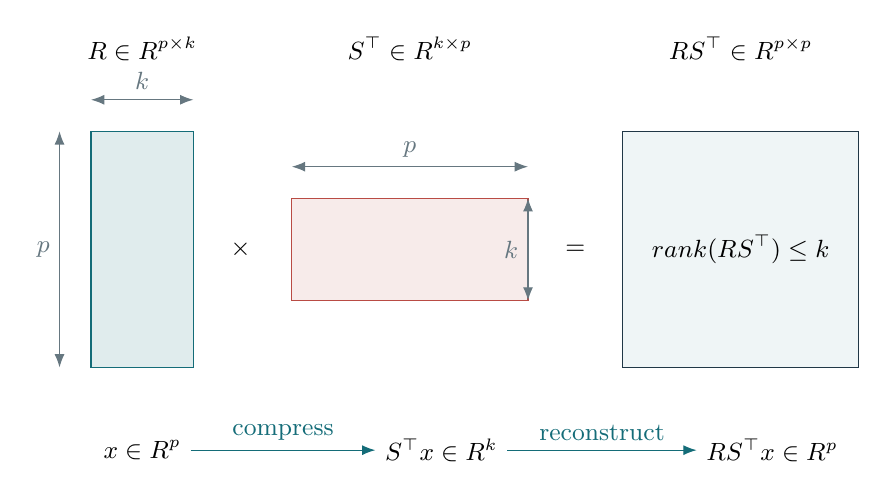
\begin{tikzpicture}[x=1cm,y=1cm]
\node at (1,4.05) {$R\in\mathbb R^{p\times k}$};
\node at (4.4,4.05) {$S^\top\in\mathbb R^{k\times p}$};
\node at (8.6,4.05) {$RS^\top\in\mathbb R^{p\times p}$};
\filldraw[fill=accent!13,draw=accent] (.35,0) rectangle(1.65,3);
\filldraw[fill=signalred!11,draw=signalred] (2.9,.85) rectangle(5.9,2.15);
\filldraw[fill=accent!7,draw=ink] (7.1,0) rectangle(10.1,3);
\node at (2.25,1.5) {$\times$};\node at (6.5,1.5) {$=$};
\draw[<->,muted] (.35,3.4)--(1.65,3.4) node[midway,above] {$k$};
\draw[<->,muted] (-.05,0)--(-.05,3) node[midway,left] {$p$};
\draw[<->,muted] (2.9,2.55)--(5.9,2.55) node[midway,above] {$p$};
\draw[<->,muted] (5.9,.85)--(5.9,2.15) node[midway,left] {$k$};
\node at (8.6,1.5) {$\operatorname{rank}(RS^\top)\leq k$};
\node (x) at (1,-1.05) {$x\in\mathbb R^p$};
\node (z) at (4.8,-1.05) {$S^\top x\in\mathbb R^k$};
\node (r) at (9,-1.05) {$RS^\top x\in\mathbb R^p$};
\draw[->,accent] (x)--(z) node[midway,above] {compress};
\draw[->,accent] (z)--(r) node[midway,above] {reconstruct};
\end{tikzpicture}
\end{document}
